%!TEX root = ../../thesis.tex
\section{Introduction}
  A dynamical system describes how the state of a system evolves with time. Formally
  \begin{definition}
    A \textbf{discrete dynamical system} is a triple $(\NN,X,\Phi)$ with a non
    empty set $X$ (the state space) and an operation $\Phi : \NN \times X \to
    X$, so that $\Phi(0,x) = x$ and $\Phi(n,\Phi(m,x)) = \Phi(n+m, x)$. 
  \end{definition}
  Thus, a discrete dynamical system is the model of a system that evolves over discrete time steps.

  The simplest case of a discrete dynamical system is when the state space is 1-dimensional (say $X \subseteq \RR$) and 
  the transition function only depends on the previous value,
  formally $\Phi(1,x) = f(x)$ for some $f : \RR \to \RR$. 
  In this case it can be written by the recurrence relation $x_{n+1} = f(x_n)$ with initial condition $x_0 \in \RR$.
  The set of the $x_n$ is called \textbf{orbit} of the map $f$.

  In this thesis only very simple examples of dynamical systems are used. 
  A broader introduction can for example be found in \cite{katok1997introduction}.

  A chaotic system is a dynamical system that is highly sensitive to initial conditions.
  As a consequence even relatively small numerical errors made during the computation grow exponentially fast.

  A prototypical example of a chaotic system is the logistic map.
  \begin{definition}\label{def:logmap}
    The \textbf{logistic map} is given by the recurrence relation 
    $ x_{n+1} = ax_n(1-x_n) \text{ with } a,\, x_0 \in \RR$.
  \end{definition} 
  \begin{table}
    \centering 
    \begin{tabular}{ | c | c | }
    \hline
    $\textbf{a}$ & \textbf{behavior} \\\hhline{|=|=|}
    $[0,1]$ & Stabilizes at $0$ \\ \hline
    $(1,3]$ & Stabilizes at $\frac{a-1}{r}$ \\ \hline 
    $(3, \approx 3.544]$ & oscillates between $2$, $4$, $8$, $\dots$ values. \\ \hline 
    $(\approx 3.544, 4]$ & \begin{tabular}{l}For almost all initial points no oscillation with finite period. \\ Small changes in the initial point yield large differences over the iterations. \end{tabular} \\ \hline
    $(4, \infty)$ & The values eventually leave the interval [0,1] and diverge for almost all initial points \\ 
    \hline
    \end{tabular}
    \caption{behavior of iterating the logistic map for different values of the parameter $a$}\label{table:logmapbehaviour}
  \end{table}
  \begin{figure}
    \centering
    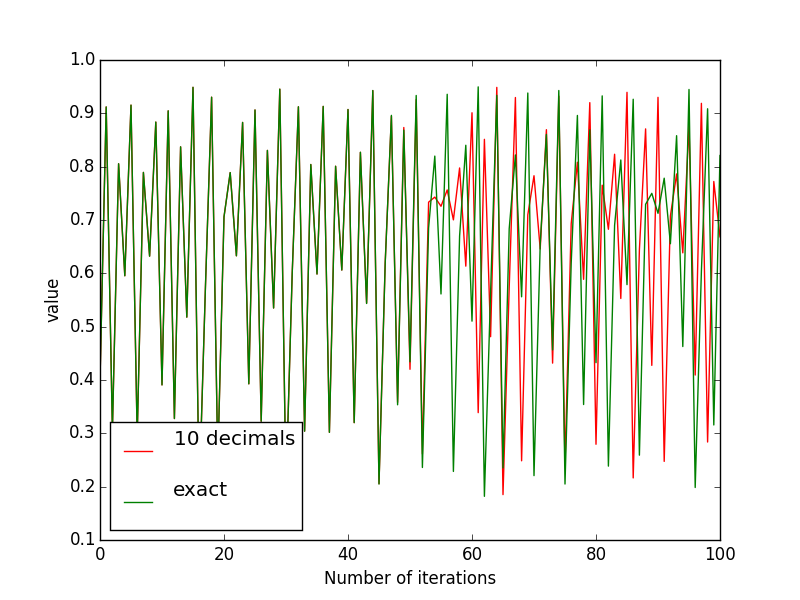
\includegraphics[width=0.5\textwidth]{img/dynamic_systems/logmap1}
    \caption{100 Iterations of the logistic map with $a=3.8$ and $x_0 = 0.4$ computed with 10 decimals precision and exactly.}
    \label{fig:logmaperror1}  
  \end{figure}
    \begin{figure}
    \centering
    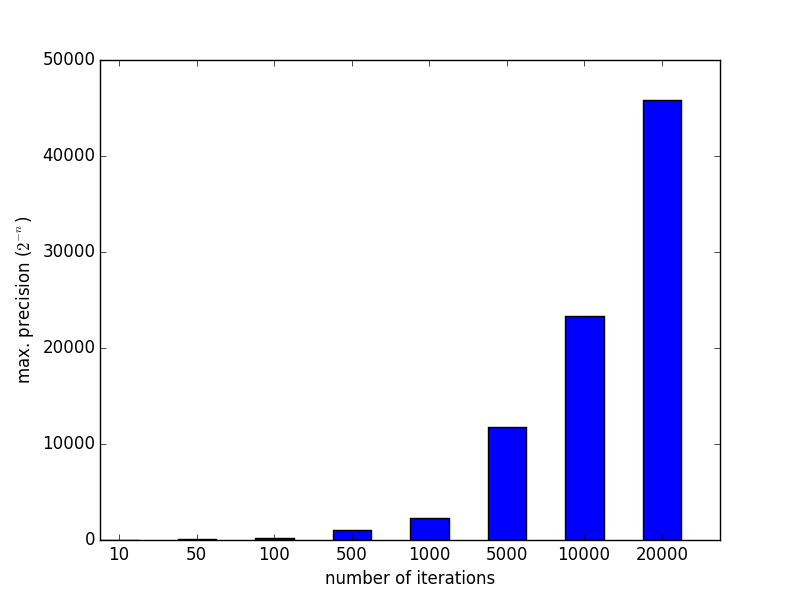
\includegraphics[width=0.5\textwidth]{img/dynamic_systems/logmap2}
    \caption{Maximal precision \irram uses to compute iterations of the logistic map and output the points with 10 decimal digits.}
    \label{fig:logmapprec}
  \end{figure}
  The behavior of the logistic map depends on the parameter $a$.\\
  Table \ref{table:logmapbehaviour} shows the behavior for different values for this parameter.

  The interesting case for this thesis is for $a \in (3.544, 4)$, since this is  where the iteration of the map leads to chaotic behavior.

  The \irram framework can be used to compute iterations of the logistic map
  exactly.
  It is therefore very well suited to investigate this chaotic behavior.
  
  Figure \ref{fig:logmaperror1} shows how sensitive the map is to small errors
  that occur because of finite precision computations.
  When using 10 significant digits for the computation, it can be seen that
  after around 50 iterations, the finite precision version diverges from the
  \irram version and after that behaves completely differently. 

  \irram can also be used to approximate the complexity in terms of needed computation precision. 
  \irram automatically increases the internal precision until it suffices to output the result with the demanded number of digits.
  Thus, the internal precision at the end of the computation gives a measure of this complexity. 

  As can be seen in Figure \ref{fig:logmapprec}, the needed internal precision
  grows extremely quickly with the number of iterations.  
  To compute 10 significant digits of the $20000$-th iterate, \irram internally
  computes already with precision nearly $2^{-50000}$, which is of course far
  from what is possible with any standard floating point data type.   
  \subsection{The Shadowing Lemma}
    The next section deals with the relation between exactly computed and approximately computed orbits and how much numerical orbits have to do with real orbits. 
    \begin{definition}\label{def:pseudoorbit}
      A sequence $(x_i)_{i \in \NN}$ is called an \textbf{$\alpha$-pseudo-orbit} for a map $f$ if for all $i \in \NN$
      $$ \| x_{i+1} - f(x_i) \| < \alpha $$  
    \end{definition}
    One can think of a pseudo orbit as a numerically computed orbit, where small rounding errors can occur in every evaluation of $f$.
    \begin{definition}\label{def:shadowing}
      A real orbit $(y_i)_{i \in \NN}$ \textbf{$\beta$-shadows} the pseudo-orbit $(x_i)_{i \in \NN}$ if for all $i \in \NN$
      $$\| x_i - y_i \| < \beta.$$  
    \end{definition}
    % \begin{definition}
    %   A dynamic system is called \textbf{uniformly hyperbolic} if ...
    % \end{definition}
    For systems that have a certain property, namely being uniformly
    hyperbolic, Anosov and Bowen could show the following result \cite{anosov1967} \cite{Bowen1975} \cite{Hasselblatt:2008}:
    \begin{theorem}[Shadowing Lemma]
     Let $f: \RR \to \RR$ be a uniformly hyperbolic map.
     Then it holds that for all $\beta > 0$ there exists an $\alpha > 0$ such that for every $\alpha$-pseudo-orbit $(x_i)_{i \in \NN}$
     there is a point $p_0$ so that the real orbit $(y_i)_{i \in \NN}$ defined by $y_0 := p_0$ and $y_{i+1} := f(y_i)$ $\beta$-shadows $(x_i)_{i \in \NN}$.
    \end{theorem} 
    In other words, in the uniformly hyperbolic case, every numerically computed orbit is close to a true orbit with a slightly changed initial point.

    Unfortunately, many maps including the logistic map, are not uniformly hyperbolic. 

    For non-hyperbolic $f$, it can not be expected, that there is a real orbit that stays close to the pseudo orbit forever.
    Instead, there will be an orbit staying close to $(x_i)$ for some time (say up to some point $n_0$) and then starting to diverge. 

    The goal of this the case study is to investigate such orbits, in
    particular to find out how long there is an orbit staying close to the
    pseudo orbit. 
    The basis for this case study is a paper by Hammel, Yorke
    and Grebogi from 1987 \cite{Hammel1987}.
    The paper deals with the question, how long numerical orbits of the logistic map can be shadowed by true orbits.

    The authors show that for $a = 3.8$ and $x_0 = 0.4$, there is a true orbit $(y_i)_{i \in \NN}$ of the logistic map, so that $\| x_n - y_n \| < 10^{-7}$ for $n \leq 10^7$.

    Their proof method is to compute bounds on the points of the true orbit with a computer by using a form of interval arithmetics. 
    All their computations were done on a Cray X-MP supercomputer. 

    For the case study, first their algorithm was implemented on a modern
    computer in the \cc programming language, both using fixed precision
    floating point numbers and \irram. 

    As a second step \irram was used to compute the shadowing orbit exactly.
  \subsection{The Algorithm}
    In their paper Hammel, Yorke and Grebogi give an algorithm to compute a
    shadowing orbit $(y_i)_{i \in \NN}$ of size $N$ for a given pseudo orbit
    $(x_n)_{n \in \NN}$ of the logistic map $f$.

    Instead of computing the shadowing orbit from the first point, the
    algorithm computes the inverse orbit by starting with the last point and
    then iteratively computing the predecessor.  Since the logistic map is not
    injective, there is not a unique choice for this predecessor. 

    For some point $f(x)$ there are normally two possible values for the
    inverse given by $$f^{-1}_{1,2}(x) = 0.5 \pm \sqrt{0.25 + \frac{x}{a}} $$

    An orbit can be computed by setting $y_N = x_N$ and then iteratively
    applying one of the inverse maps $y_{n-1} = f^{-1}(y_n)$.  

    To stay close to the pseudo orbit, in every step the point on the same side
    of $0.5$ as $x_n$ is chosen.
    In the following, this function will just be denoted by $f^{-1}$ when the choice of index is
    obvious.
    
    The backward procedure will give an orbit close to the pseudo-orbit since the
    inverse function on $(0,1)$ is a contraction, i.e. $\| f^{-1}(x) -
    f^{-1}(y) \| \leq |x-y|$. 

    Let $\delta$ be the rounding error made when numerically computing
    $f(x_n)$.
    Then it holds $\|f^{-1}(x_n)\| = \| f^{-1}(f(x_{n-1})+\delta)\| \leq \|f(x_n)\| +
    \varepsilon$ for some small $\varepsilon$.   
    This leads to
    $$ \| x_{n-1} - y_{n-1} \| = \| x_{n-1} - f^{-1}(y_n) \| \leq \|
    f^{-1}(x_n) - f^{-1}(y_n) \| + \| f^{-1}(x_n) - x_{n-1} \| \leq \| x_n -
    y_n \| + \varepsilon $$   

    Of course, using only floating point arithmetics, the inverse can not be
    computed exactly and thus the shadowing orbit itself can not be computed.

    Instead of computing the orbit, an error bound can be computed with the
    help of interval arithmetics. 
    That is, a sequence of intervals $(I_n)_{0 \leq n \leq N}$ giving upper and
    lower bounds for $y_n$ is computed, i.e Intervals $I_n$ such that
    $$y_n \in I_n \text{ for } 0 \leq n \leq N.$$

    The procedure is started with $I_N := [x_n, x_n]$ and then $I_{n-1}$ is
    selected so that $I_n \subseteq f(I_{n-1})$ holds.\\
    In each step, $I_n$ is chosen as small as possible. 

    If at some point $x_n < \frac{a}{4}$ the inverse is not defined and the
    procedure fails.
    
    In the other case, an upper bound on the maximal distance between all points in
    $I_n := [l_n, r_n]$ and $x_n$ is computed.

    That is
    $$ \delta = \max_{0 \leq n \leq N} \min(|x_n-l_i|,\, |x_n - r_i|)$$
    gives a shadowing bound.
%    \subsection{Forward Algorithm}
%    An alternative to the algorithm descriped above can be found in \cite{chow1991}.
%    Instead of starting from the last point in the pseudo orbit and going backwards, this algorithm proceeds in forward direction.
%    They define the two quantities
%    \begin{eqnarray*}
%    \sigma & = & \sup^N_{n=0} \sum_{m=n}^N  \prod_{j=n}^{m} | Df(y_j)^{-1} |  \\
%    \tau & = & \sup^N_{n=0} | \sum_{m=n}^N (y_{m+1}-f(y_m)\prod_{j=n}^{m} Df(y_j)^{-1}  |
%    \end{eqnarray*}
%    and show the following theorem:
%    \begin{theorem}
%    Let $f: [0,1] \to [0,1] \in C^2$ and $M = sup \{|D^2f(x)| \,:\, x \in [0,1] \}$.
%    For a pseudo orbit $(y_n)_{n=0}^{N+1}$ with $2M\sigma\tau \leq 1$, there is an exact orbit $(x_n)_{n=0}^N$  with 
%    $$sup_{n=0}^N |x_n - y_n| \in [\frac{tau}{1+0.5(1+\sqrt{1-2M\sigma \tau})}, \frac{2\tau}{1+\sqrt {1-2M\sigma \tau}}]$$
%    \end{theorem}
%    Then they derive the following esitmations for $\sigma$ and $\tau$:
%    The procedure to determine how closely a given pseudo orbit $(y_n)$ is shadowed by a true orbit is then given as follows:
%    \begin{enumerate}
%      \item Find upper bounds for $M$, $\delta$ and $\Delta$.
%      \item Compute 
%      \begin{eqnarray*}
%      \mu_p &=& \sup_{n=0}^{N-p} \prod_{m=n}^{n+p} |Df(y_m)^-1| \\
%      \sigma_p &=& \sup_{n=0}{N} \sum_{m=n}^{min(n+p,N)} \prod_{j=n}^{m} |Df(y_j)^-1| \\
%      \tau_p &=& \sup_{n=0}{N} \sum_{m=n}^{min(n+p,N)} \prod_{j=n}^{m} |Df(y_j)^-1| \\
%      \end{eqnarray*}
%    \end{enumerate}
\section{Implementation}
  Several versions of the above algorithm were implemented.

  The first one is a reimplementation of the original interval arithmetic version
  on a modern computer.
  
  The Cray-MP's floating point data types had different sizes than the
  standard types in modern programming languages.
  To get similar results as in the original work,  the cray double precision
  data type therefore had to be simulated using software implementations.
  
  For the \cc implementation, the boost multiprecision library \cite{boostmultiprecision} was used. 
  The library provides data types that replace the native \cc floating point types, but with a user defined precision. 
 
  The cray double data type used for the computations in the paper has machine epsilon
  $\varepsilon_\mu = 2^{-95}$.

  To compute the intervals $I_n$ from $I_{n+1}$, the inverse of the interval is
  computed as described above. 
  As long as the condition 
  \begin{equation}\label{eqn:nesting condition}  
    I_{n+1} \subseteq f(I_n) 
  \end{equation}
  is not fulfilled, $I_n$ is enlarged on both sides by the minimal possible quantity $\varepsilon_\mu$. 

  However, since both the computation of $f(I_n)$ and $f^{-1}(I_n)$ are done using
  floating point arithmetics, this is not enough to guarantee the condition
  \ref{eqn:nesting condition}.
  
  Further enlarging the interval on both sides by the constant $10^{-25}$
  takes care of this problem.
  
  For the interval arithmetic a simple interval class template
  \code{fixed\_precision\_interval<prec>} was written to represent
  intervals of the form $[a,b]$ with $a$ and $b$ multiprecision floating point
  numbers with \code{prec} bits precision. 

  All needed operations on intervals were implemented for this class, making
  the implementation of the algorithm straight forward.

  Instead of only implementing the algorithm in the original form, generic
  types where used such that different floating point precisions could be
  tried.

  The second implementation made is very similar to the first one but instead
  of using intervals with fixed precision floating point end points, \irram's
  \code{INTERVAL} type was used.

  The data type provides interval arithmetic for intervals with real numbered end points. 
  The above algorithm can therefore be implemented by first computing a pseudo
  orbit using floating point arithmetics and then computing the inverse of a
  small interval around the last point exactly.

  The last implementation uses \irram to compute a shadowing orbit exactly.

  Again, a pseudo orbit is computed by using floating point arithmetic in the
  iterations of the logistic map.

  Then, starting with the last point of the pseudo orbit the inverses can be computed exactly until the initial point is reached.
  In the end, the distance of this real orbit and the pseudo orbit can be
  computed and the maximum of all those distances taken to find the shadowing
  distance.

  One advantage of the last approach is, that the \irram code to compute the exact orbit is extremely simple. 
  Since all operations can be performed exactly there is no need for intervals
  or other complicated structures. 
  The data type real takes care of everything.

  Again, the implementation uses generic types, to make it possible to compute
  the shadowing distance for various different floating point precisions.
\section{Evaluation}
  \subsection{Breakdown points}
  As mentioned above, the algorithm only works if at each step $x_i \leq
  \frac{a}{4}$.  
  If the algorithm fails, the first $N$ for that there is some $i$ such that
  $x_i > a_i$ is called the breakdown point.

  The breakdown point depends on the precision that is used to compute the pseudo orbit. 
  \begin{figure}[h]
    \centering
    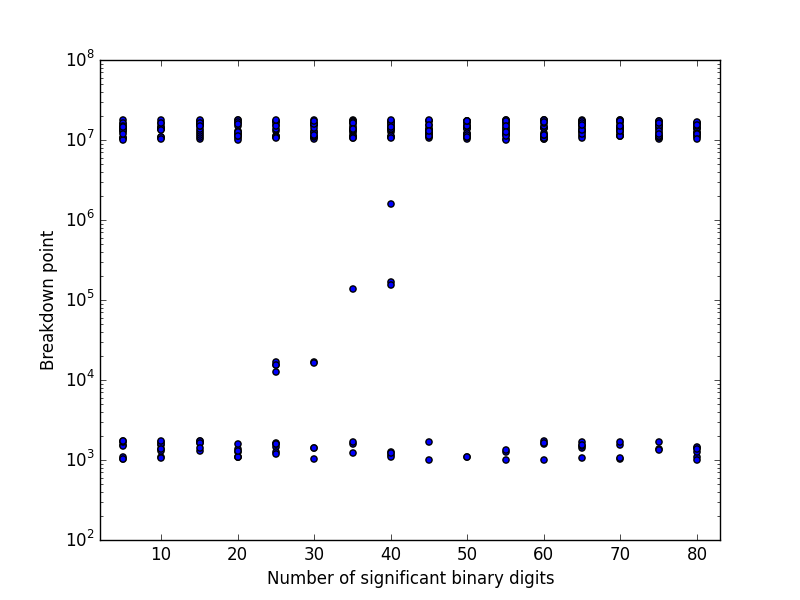
\includegraphics[width=0.6\textwidth]{img/dynamic_systems/breakdown}
    \caption{Breakdown points depending on $N$ for different parameters $a$ and
    $p_0$}\label{fig:breakdown}
  \end{figure}

  Since the computation precision on the Clay X-MP was determined by the
  available floating point data types, it was not possible to just adjust it.

  Instead, the noise was artificially increased by setting $x_{n+1} =
  ax_n(a-x_n)+\delta_p \cos (\Theta)$ with $\Theta = n (mod 997)$ and then the
  shadowing distance in relation to $\delta_p$ measured.  
  
  However, using the boost multiprecision library's \code{cpp\_bin\_float} data
  type, it is easy to change the number of binary digits of the used floating
  point data type instead of artificially increasing the noise.

  In the original work the relation $N \approx \frac{1}{\sqrt \delta_p}$
  between the noise amplitude and the breakdown points was found.

  Interestingly no such relation could be found for the modified version that
  uses \code{cpp\_bin\_float} instead of a noise amplitude.
  As can be seen in \ref{fig:breakdown}, in this version breakdowns very rarely
  occur at all during the first $10^7$ iterations.
  There are, however, still some parameters for that a breakdown occurs.
  In most of this cases it occurs rather quickly, during the first 1000 iterates.

  The reason for that is probably that the correct rounding compensates much
  of the errors, which is not the case when the noise is artificially generated
  by the noise amplitude.

  \subsection{Shadowing bound and computation precision}
  The original paper also deals with the question, how close a pseudo-orbit is
  shadowed depending on the computation precision. 
  The same was also done for the different implementations in this thesis.

  Again, instead of artificially generating noise, the precision of the
  floating point type was changed.

  \begin{figure}[H]
    \centering
    \begin{subfigure}{.45\textwidth}
      \centering
      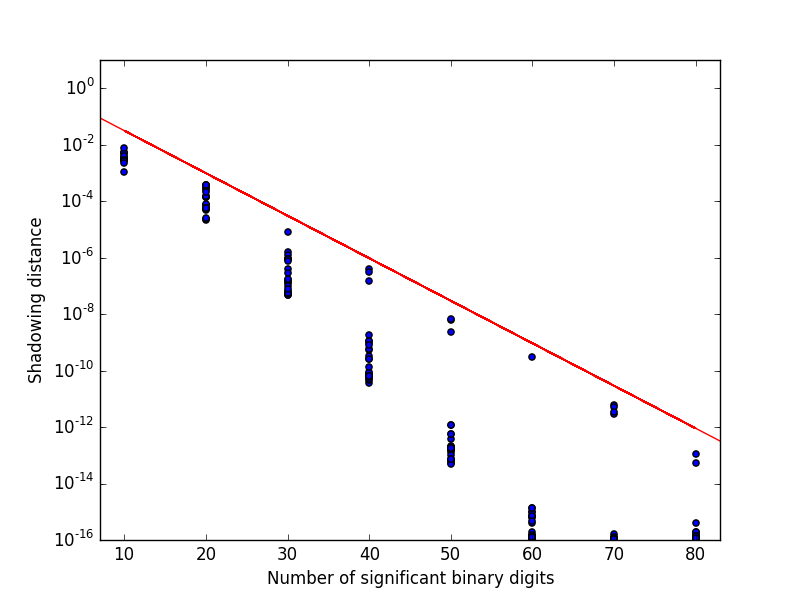
\includegraphics[width=1.0\textwidth]{img/dynamic_systems/dist_prec_N_1000}
      \caption{$10^3$ iterations}
    \end{subfigure}
     \begin{subfigure}{.45\textwidth}
      \centering
      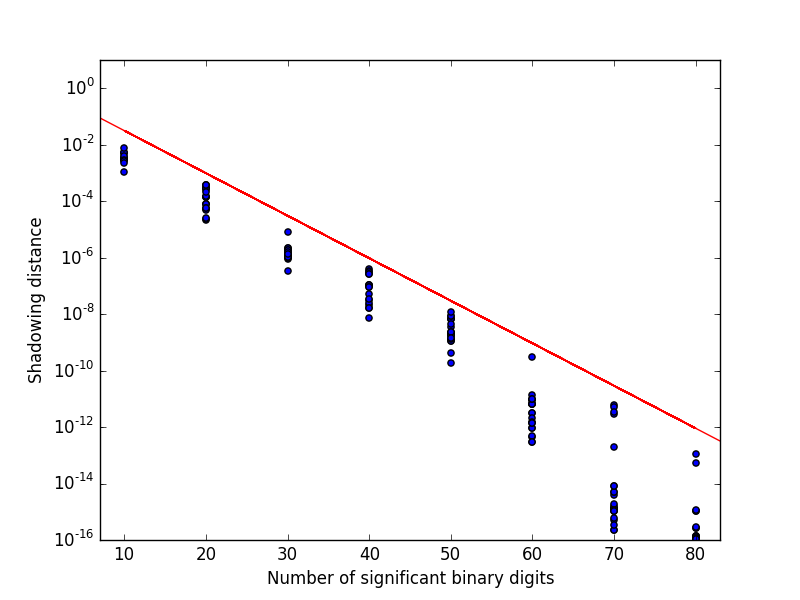
\includegraphics[width=1.0\textwidth]{img/dynamic_systems/dist_prec_N_10000000}
      \caption{$10^7$ iterations}
    \end{subfigure}   
    \caption{Shadowing distance for different parameters $a$ and $p_0$ of the  logistic map. The distance is bound by $\frac1{\sqrt \delta}$ where $\delta = 2^{-n}$ is the precision.}
    \label{fig:shadowingdistance1}
  \end{figure}

  The shadowing distance was computed for several different parameters $a$ and starting points $p_0$. 
  The number of iterations $N$ were also varied. 

  The result can be seen in Figure \ref{fig:shadowingdistance1}. 
  
  The tests were made with all versions of the algorithm described above.
  The results obtained from the different versions were nearly identical, thus
  only the \irram version is depicted.
  Also, the running time of both program versions did not differ much for
  the performed  evaluations.
  %A complete table of all the starting values and parameters can be found in
  %the Appendix. 

  In the original paper it is conjectured that for $2M$-digit
  accuracy, that the orbit stays close to $10^{-M}$ for around $10^M$ iterates.

  As can be seen in the graph, for up to $10^7$ iterates the conjecture holds. 
